\begin{tikzpicture}[scale=1,inner sep=0.4mm]
\node at (0,0) {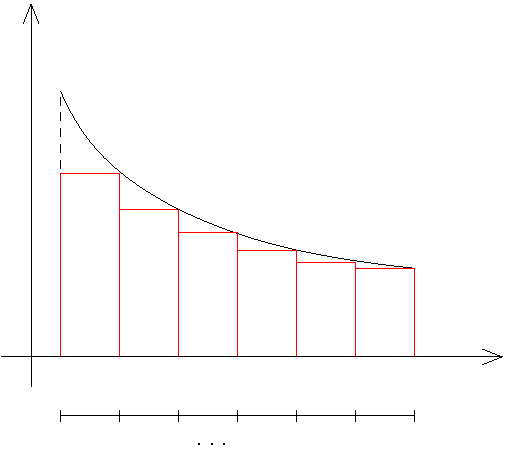
\includegraphics[scale=1]{/home/marcin/dydaktyka/latex/przyklady/metoda-prostokatow.pdf}};
\node at (0,2) {$\int_{a}^{b}f(x) dx \approx h \sum_{i=1}^{n}f(x_i)$};
\node at (-3.2,-2.4) {$x_0 = a$};
\node at (-0.2,-2.4) {$x_i$};
\node at (2.8,-2.4) {$x_n = b$};
\node at (-2.7,-3.4) {$h$};
\node at (-1.8,-3.4) {$h$};
\node at (1.8,-0.2) {$y=f(x)$};
\node[blue] at (0,2.8) {Przyk\l{}ad rysunku z na\l{}o\.zonymi wzorami};
\end{tikzpicture}